\chapter{परिवर्धनी आनुवंशिकी और आकार का विकास}\label{ch:b3:developmental-genetics}

किसी फल-मक्खी का अंडा आधा मिलीमीटर लंबा है, और निषेचन के बाद के तीन
घंटों में, इससे पहले कि उसके छह हज़ार केंद्रकों के बीच कोई एक भी
कोशिका-झिल्ली बने, वह तय कर लेता है कि कौन-सा सिरा सिर होगा, कौन-सा
पूँछ, चौदह खंडों में से हर एक कहाँ पड़ेगा, और उनमें से कौन टाँगें, पंख
या स्पर्शश्रृंग ढोएगा। वह यह कुछ दर्जन जीनों से करता है, जो पट्टियों की
किसी उत्तरोत्तर महीन होती पदानुक्रमी में चालू होते हैं, और हर पट्टी अपने
से पहले की पट्टियों के उत्पादों की सांद्रताओं से पढ़ी जाती है। 1980 में
हाइडेलबर्ग के दो नौजवान वैज्ञानिकों ने हज़ारों उत्परिवर्ती मक्खियाँ ऐसे
डिंभकों के लिए छानीं जिनके अंग ग़ायब या दुहरे हों, और उन्हें पूरी
पदानुक्रमी मिल गई: वे जीन जिनके खोने से खंडों का कोई गुच्छा मिट जाता है,
वे जिनके खोने से हर दूसरा खंड मिट जाता है, और वे जिनके खोने से हर खंड
आगे-पीछे उलट जाता है। उसी वर्ष के उस काम ने, जो किसी ऐसे जीन पर था जो
मक्खी के तीसरे खंड को उसके दूसरे की नक़ल में बदल देता है --- और उसे चार
पंख दे देता है, जैसे उसके पूर्वजों के थे --- ऐसे स्वामी जीनों का कोई
समुच्चय खोल दिया जो, जैसा पता चला, किसी चूहे और किसी मनुष्य के
गुणसूत्रों पर भी उसी क्रम में पड़े थे और वही काम करते थे। यह अध्याय इस
बारे में है कि कोई भ्रूण अपनी ही ज्यामिति कैसे गणित करता है, कुछ सौ
नियामक जीन हर प्राणी-शरीर कैसे बनाते हैं, और उनके कब तथा कहाँ काम करने
को बदलने से प्राणी-आकार की विविधता कैसे बनी है।

\section{मक्खी के निर्देशांक}

\begin{definition}[खंडन-पदानुक्रमी]\label{def:b3:developmental-genetics:hierarchy}
\index{मातृ-प्रभाव जीन}\index{रिक्ति जीन}\index{युग्म-नियम जीन}\index{खंड-ध्रुवता जीन}\index{संकोशिकीय कोरकचर्म}
\emph{Drosophila} का भ्रूण अपने पहले तेरह केंद्रक-विभाजनों तक किसी
\emph{संकोशिकीय कोरकचर्म} की तरह विकसित होता है, यानी ऐसी एक ही कोशिका
की तरह जिसके केंद्रक एक ही कोशिकाद्रव्य साझा करते हैं, इसलिए प्रोटीन
वहाँ से, जहाँ वे बनते हैं, स्वच्छंद विसरित होते हैं। माँ की कोशिकाओं की
बिछाई चार प्रवणताएँ वे अक्ष तय करती हैं: \emph{bicoid} का mRNA अग्र
ध्रुव पर बँधा है और उसका प्रोटीन पीछे की ओर विसरित होकर सिर से पूँछ तक
कोई चरघातांकी प्रवणता बनाता है; पश्च ध्रुव पर \emph{nanos} का mRNA
दर्पण-प्रवणता बनाता है; \emph{hunchback} और \emph{caudal} के mRNA
एकसमान हैं, पर Bicoid प्रोटीन \emph{caudal} का अनुवादन दबाता है और
Nanos \emph{hunchback} का, इसलिए उनके प्रोटीन भी प्रवणताएँ बनाते हैं।
ये \emph{मातृ-प्रभाव} उत्पाद, जिनका उत्परिवर्ती लक्षणरूप भ्रूण के नहीं
बल्कि माँ के जीनरूप पर निर्भर है, \emph{रिक्ति जीन}
(\emph{hunchback}, \emph{Krüppel}, \emph{knirps}, \emph{giant}) चौड़ी
पट्टियों में चालू करते हैं, जिनमें हर एक Bicoid की सांद्रता की किसी
परास पर अनुक्रिया देता है और अपने पड़ोसियों को दबाता है; रिक्ति-प्रोटीन,
संयोजन में, \emph{युग्म-नियम जीन} (\emph{even-skipped}, \emph{fushi
tarazu}, \emph{hairy}) हर एक को सात-सात पट्टियों में, बारी-बारी, चालू
करते हैं; और युग्म-नियम प्रोटीन \emph{खंड-ध्रुवता जीन}
(\emph{engrailed}, \emph{wingless}, \emph{hedgehog}) चौदह पट्टियों में,
प्रति खंड एक, चालू करते हैं, जो हर खंड का आगा और पीछा तय करते हैं और
कोशिकाएँ बन जाने के बाद उनके बीच के संकेतन से बनाए रखे जाते हैं। तीन
घंटे, चार तहें, किसी एक प्रवणता से चौदह खंडों तक --- और उन उत्परिवर्ती
नामों में वह छानबीन दर्ज है: \emph{hunchback} में वक्ष नहीं,
\emph{Krüppel} (``लँगड़ा'') में बीच का हिस्सा, \emph{fushi tarazu}
(``पर्याप्त खंड नहीं'') में हर दूसरा खंड, और \emph{hedgehog} में
शूकों की कोई चादर।
\end{definition}

\begin{omfigure}
\begin{tikzpicture}[every node/.style={font=\scriptsize}, >=stealth]
  \foreach \y/\lab/\n in {0/{मातृ: Bicoid प्रवणता}/1, -1.3/{रिक्ति जीन: 4 चौड़ी पट्टियाँ}/2, -2.6/{युग्म-नियम जीन: 7 पट्टियाँ}/3, -3.9/{खंड-ध्रुवता: 14 पट्टियाँ}/4} {
    \draw[thick, gray!60] (0,\y) ellipse (3.6 and 0.5);
    \node[left, align=right] at (-3.8,\y) {\lab};
  }
  % bicoid gradient shading
  \begin{scope}
    \clip (0,0) ellipse (3.6 and 0.5);
    \shade[left color=omDef!80, right color=omDef!2] (-3.6,-0.5) rectangle (3.6,0.5);
  \end{scope}
  \node[right, font=\tiny] at (3.7,0) {अग्र में ऊँचा};
  % gap bands
  \begin{scope}
    \clip (0,-1.3) ellipse (3.6 and 0.5);
    \fill[omDef!50] (-3.4,-1.8) rectangle (-1.6,-0.8); \fill[omThm!40] (-1.4,-1.8) rectangle (0.2,-0.8); \fill[omMeth!40] (0.4,-1.8) rectangle (1.7,-0.8); \fill[omProp!45] (1.9,-1.8) rectangle (3.4,-0.8);
  \end{scope}
  \node[font=\tiny] at (-2.5,-1.3) {\emph{hb}}; \node[font=\tiny] at (-0.6,-1.3) {\emph{Kr}}; \node[font=\tiny] at (1.05,-1.3) {\emph{kni}}; \node[font=\tiny] at (2.65,-1.3) {\emph{gt}};
  % pair-rule stripes
  \begin{scope}
    \clip (0,-2.6) ellipse (3.6 and 0.5);
    \foreach \i in {0,...,6} { \fill[omThm!50] ({-3.1+\i*0.9},-3.1) rectangle ({-2.75+\i*0.9},-2.1); }
  \end{scope}
  \node[right, font=\tiny] at (3.7,-2.6) {\emph{eve}, हर दूसरा खंड};
  % segment polarity stripes
  \begin{scope}
    \clip (0,-3.9) ellipse (3.6 and 0.5);
    \foreach \i in {0,...,13} { \fill[omProp!60] ({-3.25+\i*0.47},-4.4) rectangle ({-3.1+\i*0.47},-3.4); }
  \end{scope}
  \node[right, font=\tiny] at (3.7,-3.9) {\emph{en}: प्रति खंड एक};
  \foreach \y in {-0.55,-1.85,-3.15} { \draw[->, thick] (0,\y) -- (0,\y-0.2); }
  \node[below, align=center, font=\tiny] at (0,-4.5) {हर तह अपने ऊपर की तह की सांद्रताएँ पढ़ती है;\\किसी एक प्रवणता से चौदह खंडों तक तीन घंटे};
\end{tikzpicture}

{\small खंडन-पदानुक्रमी। कोई मातृ प्रवणता चार रिक्ति-जीन पट्टियों में
पढ़ी जाती है; रिक्ति-प्रोटीन, संयोजन में, सात युग्म-नियम पट्टियों में;
और वे चौदह खंड-ध्रुवता पट्टियों में। हर पट्टी कोई ऐसी सीमा है जो वहाँ
खींची जाती है जहाँ कोई सांद्रता किसी देहली को पार करती है।}
\end{omfigure}

\begin{theorem}[संश्लेषण, विसरण और क्षय से बनी कोई आकारजन-प्रवणता]\label{thm:b3:developmental-genetics:gradient}
\index{आकारजन}\index{स्थानिक सूचना}\index{फ़्रांसीसी झंडा प्रतिरूप}\index{क्षय-लंबाई}
किसी ऊतक के एक सिरे पर दर $J$ (प्रति एकांक क्षेत्रफल) से बनता,
गुणांक $D$ से विसरित होता और दर-अचर $k$ से अपघटित होता कोई प्रोटीन
किसी ऐसी स्थायी अवस्था तक पहुँचता है जिसमें अक्ष $x$ के अनुदिश उसकी
सांद्रता यह मानती है
\[
D\,\frac{\mathrm{d}^{2}c}{\mathrm{d}x^{2}} - k\,c = 0,
\qquad c(x) = c_{0}\,\mathrm{e}^{-x/\lambda}, \qquad \lambda = \sqrt{D/k},
\quad c_{0} = \frac{J}{\sqrt{Dk}} .
\]
\emph{\omterm{thm:b3:developmental-genetics:gradient}{क्षय-लंबाई}} $\lambda$ उस प्रवणता की पहुँच तय करती है; कोई कोशिका
अपनी स्थिति $c$ की देहलियों से तुलना करके पढ़ती है --- वॉलपर्ट (1969)
का \emph{फ़्रांसीसी झंडा}: $T_{1}$ के ऊपर नीला, $T_{1}$ तथा
$T_{2}$ के बीच सफ़ेद, नीचे लाल --- और देहली $T$ की सीमा
$x_{T} = \lambda\ln(c_{0}/T)$ पर पड़ती है। दो परिणाम: स्रोत दुगुना करने
से हर सीमा उतने ही $\lambda\ln 2$ से पीछे खिसक जाती है, और उस सांद्रता
को पढ़ने में कोई भिन्नात्मक त्रुटि $\delta c/c$ कोई स्थानिक त्रुटि
$\delta x = \lambda\,\delta c/c$ है, इसलिए कोई प्रवणता किसी सीमा को
कोशिका भर के भीतर तभी रख सकती है जब वे कोशिकाएँ उसे कुछ ही प्रतिशत के
भीतर पढ़ें। \qty{500}{\micro m} के किसी अंडे में Bicoid का
$\lambda \approx \qty{100}{\micro m}$ है: वह प्रवणता
$\mathrm{e}^{5}
\approx 150$ के किसी गुणक भर फैली है, और \emph{hunchback} की सीमा
अंडे के बीच पड़ती है, जहाँ Bicoid गिरकर अपने शिखर का लगभग बारहवाँ भाग रह
जाता है।
\end{theorem}
\begin{proof}
$x$ और $x + \mathrm{d}x$ के बीच किसी पट्ट में संरक्षण: स्थायी अवस्था पर
शुद्ध विसरणी अंतर्वाह $D\,\partial^{2}c/\partial x^{2}$ अपघटन $kc$ को
संतुलित करता है, जिससे वह समीकरण मिलता है; और $x \to \infty$ पर परिबद्ध
हल वही क्षय होता चरघातांक है, जिसमें
$\lambda^{2} = D/k$। स्रोत: $x = 0$ पर विसरणी फ्लक्स, $-D\,
c'(0) = Dc_{0}/\lambda$, $J$ के बराबर है, इसलिए $c_{0} = J\lambda/D =
J/\sqrt{Dk}$। देहली: $c_{0}\mathrm{e}^{-x_{T}/\lambda} = T$ से
$x_{T}$ मिलता है; और $c_{0}$ दुगुना करने से $\lambda\ln 2$ हर
$x_{T}$ में जुड़ जाता है, चाहे $T$ कुछ भी हो। त्रुटि:
$x_{T} = \lambda\ln(c_{0}/c)$ का अवकलन करने पर
$\delta x = -\lambda\,\delta c/c$। वह स्थायी अवस्था काल-मापक्रम
$1/k$ पर छू ली जाती है, जो Bicoid के लिए (\qty{50}{min}) उपलब्ध दो
घंटों के बराबर है, इसलिए वह प्रवणता तब पढ़ी जाती है जब वह जम ही रही होती
है।
\end{proof}

\begin{omfigure}
\begin{tikzpicture}
\begin{axis}[
  width=0.7\linewidth, height=5.6cm,
  axis x line=bottom, axis y line=left,
  xmin=0, xmax=500, ymin=0, ymax=1.05,
  xlabel={अग्र ध्रुव से दूरी (\unit{\micro m})}, ylabel={Bicoid, सापेक्ष},
  xlabel style={font=\small, at={(axis description cs:0.5,-0.12)}, anchor=north}, ylabel style={font=\small},
  tick label style={font=\small}, xtick={0,100,250,400,500}, ytick={0.08,0.3,0.6,1},
  yticklabels={0.08,0.3,0.6,1},
  clip=false,
]
\fill[omDef!15] (axis cs:0,0) rectangle (axis cs:120,1.05);
\fill[gray!8] (axis cs:120,0) rectangle (axis cs:250,1.05);
\fill[omThm!12] (axis cs:250,0) rectangle (axis cs:500,1.05);
\addplot[very thick, omDef, domain=0:500, samples=100] {exp(-x/100)};
\addplot[thick, omDef!50, dashed, domain=66:500, samples=100] {2*exp(-x/100)};
\draw[dashed, gray] (axis cs:0,0.3) -- (axis cs:120,0.3) -- (axis cs:120,0);
\draw[dashed, gray] (axis cs:0,0.08) -- (axis cs:250,0.08) -- (axis cs:250,0);
\node[font=\scriptsize, anchor=south] at (axis cs:60,1.0) {सिर};
\node[font=\scriptsize, anchor=south] at (axis cs:185,1.0) {वक्ष};
\node[font=\scriptsize, anchor=south] at (axis cs:375,1.0) {उदर};
\node[font=\scriptsize, omDef, anchor=west] at (axis cs:255,0.35) {$c = c_{0}\,\mathrm{e}^{-x/\lambda}$, $\lambda = \qty{100}{\micro m}$};
\node[font=\scriptsize, omDef!70!black, anchor=west, align=left] at (axis cs:255,0.62) {बिंदुदार: स्रोत दुगुना ---\\हर सीमा $\lambda\ln 2 = \qty{69}{\micro m}$ खिसकती है};
\node[font=\scriptsize, gray, anchor=north east] at (axis cs:118,0.29) {$T_{1}$};
\node[font=\scriptsize, gray, anchor=south west] at (axis cs:300,0.09) {$T_{2}$: \emph{hunchback} बंद};
\end{axis}
\end{tikzpicture}

{\small किसी चरघातांक का खींचा फ़्रांसीसी झंडा। एक ही प्रवणता पर पड़ी
देहलियाँ उस अंडे को क्षेत्रों में बाँट देती हैं; और कोई प्रबल स्रोत सारी
सीमाएँ उतनी ही दूरी पीछे सरका देता है, और यही \emph{bicoid} की अतिरिक्त
प्रतियों वाली माँओं के भ्रूण दिखाते हैं।}
\end{omfigure}

\begin{proof}[प्रमाण-सामग्री]
नुसलाइन-फ़ोलहार्ट और वीशाउस (1980) ने मक्खियों को कोई उत्परिवर्तजन
खिलाया, उनकी संतानों को समयुग्मजता तक प्रजनित किया, और कोई
\num{27000} मरे डिंभकों की उपत्वचा सूक्ष्मदर्शी के नीचे ग़ायब या
दुहराए प्रतिरूप के लिए देखी: कोई एक सौ बीस जीन, जो अपने लक्षणरूपों से
रिक्ति, युग्म-नियम और खंड-ध्रुवता वर्गों में छँट गए --- यानी कोई
पदानुक्रमी, जो किसी भी अणु के ज्ञात होने से पहले दिख गई। ड्रीवर और
नुसलाइन-फ़ोलहार्ट (1988) ने भ्रूणों को Bicoid प्रोटीन के लिए रँगा और
अग्र ध्रुव से वह चरघातांकी प्रवणता देखी; और जिन माँओं के पास उस जीन की
एक, दो, चार या छह प्रतियाँ थीं उनके भ्रूणों की प्रवणताएँ अनुपाती
ऊँचाई की थीं, और सिर की वलि तथा \emph{hunchback} की सीमा उस मात्रा के
साथ पीछे की ओर सरक गई, ठीक जैसा वह देहली-प्रतिरूप पूर्वानुमान करता है
और मोटे तौर पर प्रति दुगुनी के उसी $\lambda\ln 2$ से जितना वह माँगता
है। किसी अंडे के बीच में \emph{bicoid} का mRNA अंतःक्षिप्त करने से वहाँ
कोई सिर बन गया।
\end{proof}

\begin{omfigure}
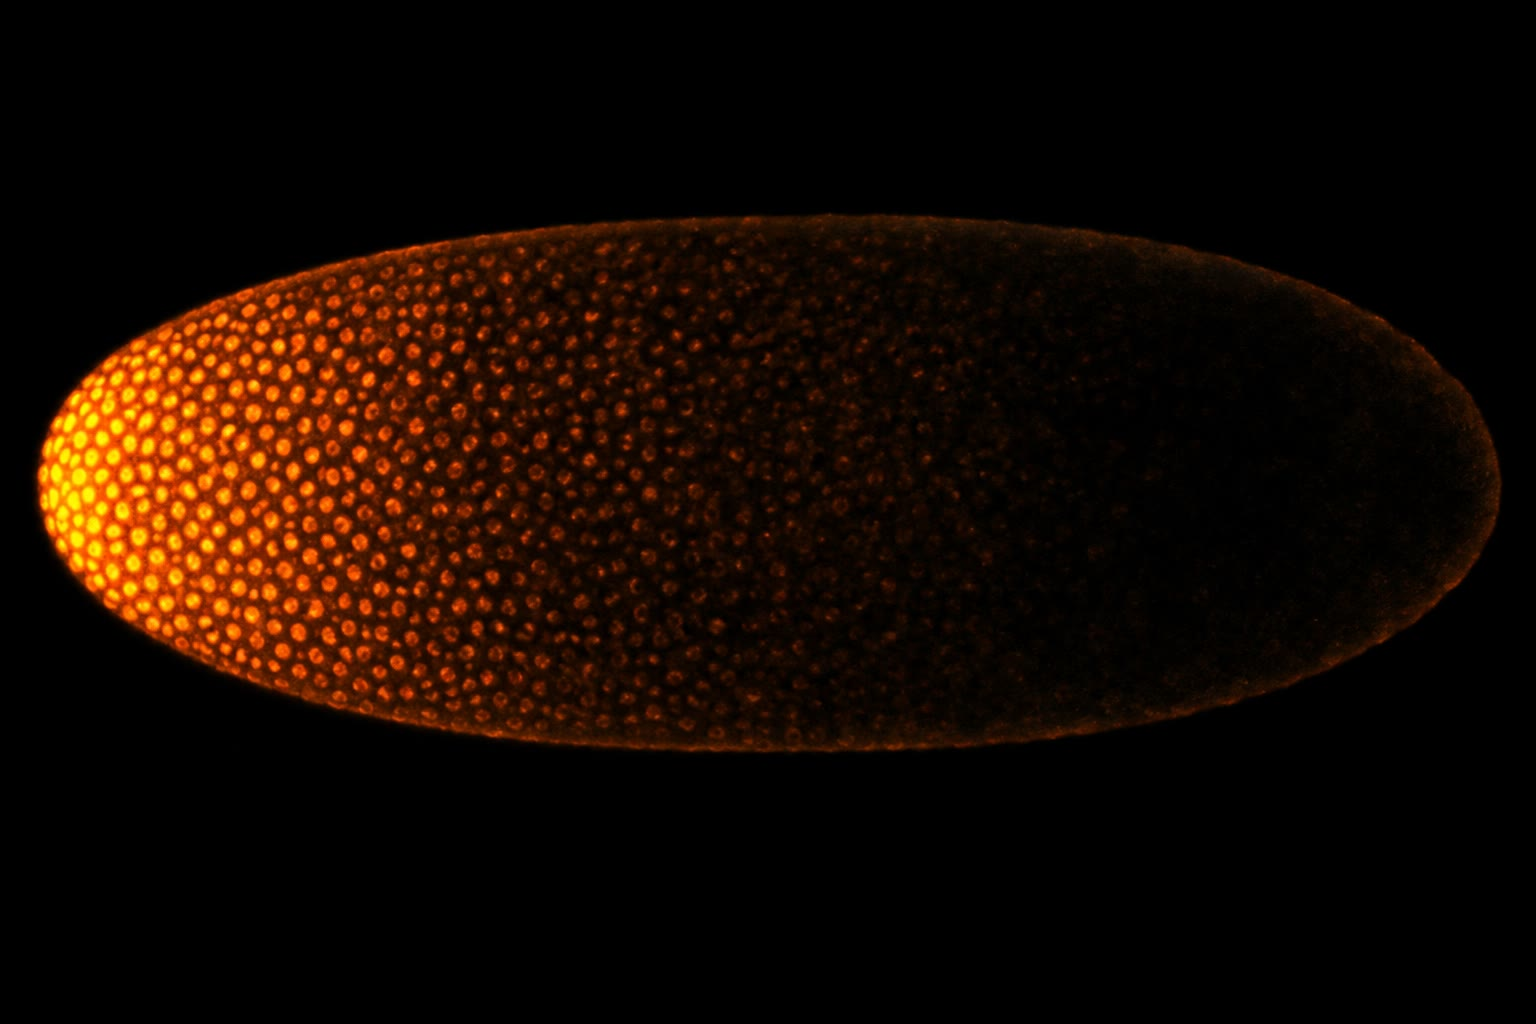
\includegraphics[width=0.46\linewidth]{images/book5/ai/b5-23-bicoid-gradient.jpg}\hspace{0.04\linewidth}
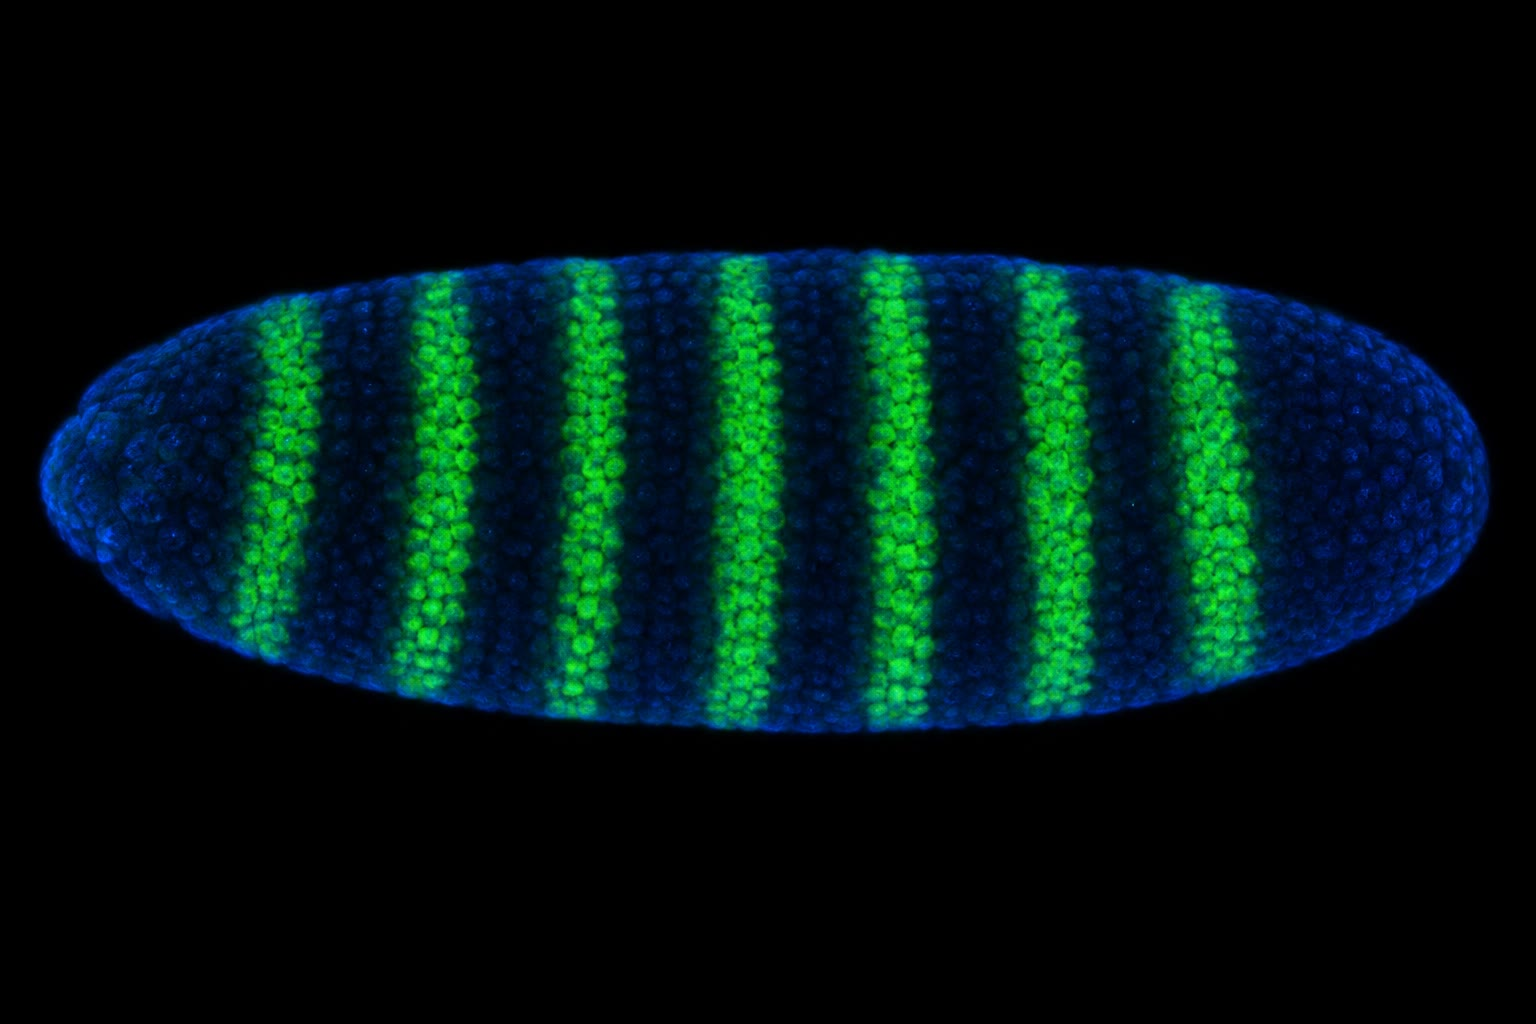
\includegraphics[width=0.46\linewidth]{images/book5/ai/b5-23-embryo-stripes.jpg}

{\small बाएँ: Bicoid प्रोटीन के लिए रँगा कोई संकोशिकीय भ्रूण, जो अग्र
ध्रुव पर सबसे चमकीला है और पश्च की ओर चरघातांकी रूप से फीका पड़ता है।
दाएँ: घंटे भर बाद किसी युग्म-नियम प्रोटीन के लिए रँगा कोई भ्रूण, जिसमें
रिक्ति-जीन पट्टियों से खींची गई सात पट्टियाँ हैं।}
\end{omfigure}

\section{पहचान: Hox जीन}

\begin{definition}[समरूपांतरी जीन और सहरैखिकता]\label{def:b3:developmental-genetics:hox}
\index{समरूपांतरी उत्परिवर्तन}\index{Hox जीन}\index{सहरैखिकता}\index{होमियोबॉक्स}\index{Hox कूट}
कोई \emph{समरूपांतरी} उत्परिवर्तन किसी एक देह-अंग को किसी दूसरे में बदल
देता है: यह बेटसन का शब्द (1894) है उन असामान्यताओं के लिए जो ``किसी
शृंखला के एक सदस्य की जगह दूसरे को रख देती हैं।'' मक्खी में
\emph{Antennapedia} के प्रभावी उत्परिवर्ती वहाँ टाँगें उगा लेते हैं जहाँ
स्पर्शश्रृंग होने चाहिए; \emph{bithorax} उत्परिवर्ती (लुइस, 1978) तीसरे
वक्षीय खंड को दूसरे की नक़ल में बदल देते हैं, जिससे वे संतुलक (हॉल्टियर)
पंखों की कोई दूसरी जोड़ी बन जाते हैं। इसके ज़िम्मेदार आठ जीन, यानी
\emph{Hox जीन}, एक ही गुणसूत्र पर दो गुच्छों में पड़े हैं, और लुइस ने
देखा कि DNA पर उनका क्रम शरीर पर उन खंडों के क्रम से मेल खाता है जिन्हें
वे नियंत्रित करते हैं --- यानी \emph{सहरैखिकता}, जिसकी व्याख्या अब भी
पूरी नहीं हुई। हर एक कोई ऐसा अनुलेखन कारक कूटबद्ध करता है जिसमें वही
60-ऐमीनो-अम्ल का DNA-बंधक \emph{होमियोबॉक्स} प्रांत है (मैकगिनिस,
गेरिंग, 1984), जो फिर हर प्राणी में मिला: चूहे और मनुष्य तेरह-तेरह जीनों
के चार गुच्छे ढोते हैं, उसी तरह सहरैखिक, जो देह-अक्ष के अनुदिश एक-दूसरे
में धँसे प्रांतों में अभिव्यक्त होते हैं, और उस गुच्छे के बाद वाले जीन
अधिक पश्च। उस अक्ष के अनुदिश किसी कोशिका की पहचान उन Hox जीनों के संयोजन
से मिलती है जिन्हें वह अभिव्यक्त करती है, यानी \emph{Hox कूट}; और पश्च
जीन अग्र जीनों पर हावी रहते हैं (पश्च प्रबलता), इसलिए किसी पश्च जीन के
खोने से वह खंड अपने आगे वाले की पहचान अपना लेता है। Hox जीन कोई खंड
बनाते नहीं; वे किसी पहले से बने खंड को बताते हैं कि वह कौन-सा है, और यह
वे किसी टाँग, पंख, पसली या कटि-कशेरुक के लायक अनुवर्ती जीनों की
बैटरियाँ चालू करके करते हैं।
\end{definition}

\begin{omfigure}
\begin{tikzpicture}[every node/.style={font=\scriptsize}, >=stealth]
  % fly cluster
  \node[left] at (-0.3,2.2) {मक्खी (\emph{Drosophila}), 8 जीन};
  \foreach \i/\g/\c in {0/lab/omDef, 1/pb/omDef, 2/Dfd/omThm, 3/Scr/omThm, 4/Antp/omMeth, 5/Ubx/omMeth, 6/abd-A/omProp, 7/Abd-B/omProp} {
    \draw[thick, fill=\c!40] ({\i*1.1},1.9) rectangle ({\i*1.1+0.9},2.5); \node[font=\tiny] at ({\i*1.1+0.45},2.2) {\emph{\g}};
  }
  \node[left] at (-0.3,0.9) {चूहे का HoxB गुच्छा, 13 में से 9};
  \foreach \i/\g/\c in {0/b1/omDef, 1/b2/omDef, 2/b3/omDef, 3/b4/omThm, 4/b5/omThm, 5/b6/omMeth, 6/b7/omMeth, 7/b8/omProp, 8/b9/omProp} {
    \draw[thick, fill=\c!40] ({\i*1.1},0.6) rectangle ({\i*1.1+0.9},1.2); \node[font=\tiny] at ({\i*1.1+0.45},0.9) {\emph{\g}};
  }
  \draw[->, thick] (0,1.55) -- (9.8,1.55); \node[above, font=\tiny] at (4.9,2.55) {DNA पर 3$'$ $\to$ 5$'$};
  \draw[->, thick] (0,0.2) -- (9.8,0.2); \node[below, font=\tiny] at (4.9,0.05) {शरीर पर अग्र $\to$ पश्च};
  % body schematic
  \node[left] at (-0.3,-0.9) {कहाँ अभिव्यक्त};
  \draw[thick, gray!70, rounded corners=6pt] (0,-1.3) rectangle (9.8,-0.5);
  \foreach \x/\t in {0.6/{सिर}, 2.6/{गर्दन}, 4.4/{वक्ष}, 6.6/{कटि}, 8.6/{त्रिक, पूँछ}} { \node[font=\tiny] at (\x,-0.9) {\t}; }
  \draw[gray!70] (1.6,-1.3) -- (1.6,-0.5); \draw[gray!70] (3.5,-1.3) -- (3.5,-0.5); \draw[gray!70] (5.6,-1.3) -- (5.6,-0.5); \draw[gray!70] (7.6,-1.3) -- (7.6,-0.5);
  \node[below, align=center, font=\tiny] at (4.9,-1.4) {सहरैखिकता: गुणसूत्र पर जीनों का क्रम शरीर पर उनके प्रांतों का क्रम है;\\वही गुच्छे, वही क्रम, मक्खी से चूहे तक ---\\जो साठ करोड़ वर्ष पहले के किसी पूर्वज से विरासत में मिले};
\end{tikzpicture}

{\small किसी मक्खी और किसी चूहे में Hox गुच्छे। वे जीन DNA पर उन्हीं
देह-क्षेत्रों के क्रम में पड़े हैं जिन्हें वे निर्दिष्ट करते हैं, दोनों
प्राणियों में, और समजात जीन अनुक्रम से पहचाने जा सकते हैं: चूहे का कोई
\emph{Hoxb6} जीन पहचानने लायक ढंग से मक्खी का \emph{Antennapedia} है।}
\end{omfigure}

\begin{proof}[प्रमाण-सामग्री]
लुइस (1978) ने \emph{bithorax} संकुल को उत्परिवर्तनों की ऐसी शृंखला की
तरह मानचित्रित किया जिनमें हर एक किसी खंड को उसके आगे वाले में बदल देता
था और जो उस गुणसूत्र पर देह-क्रम में सजे थे, और प्रस्ताव किया कि वे जीन
उस अक्ष के अनुदिश क्रमिक रूप से सक्रिय होते हैं। मैकगिनिस और सहयोगियों
(1984) ने वह \omterm{def:b3:developmental-genetics:hox}{होमियोबॉक्स} \emph{Antennapedia} तथा
\emph{Ultrabithorax} के बीच पर-संकरण से पाया और फिर मेंढकों तथा चूहों
में। वह प्रकार्यगत तुल्यता सीधे दिखाई गई: किसी मक्खी में अभिव्यक्त
चूहे का कोई \emph{Hoxb6} जीन \emph{Antennapedia} लक्षणरूप पैदा करता है,
यानी स्पर्शश्रृंगों से टाँगें (1990 का दशक); जिस चूहे में
\emph{Hoxc8} न हो उसकी पहली कटि-कशेरुका पर एक अतिरिक्त पसली होती है,
क्योंकि उस खंड ने अपने आगे वाले की पहचान ले ली; और चूज़े तथा चूहे में
Hox की अभिव्यक्ति-सीमाएँ बदलने से वह स्थान खिसक जाता है जहाँ अग्र-उपांग
बनते हैं, और किसी हंस की गर्दन की लंबाई उसी सीमा के किसी पश्च खिसकाव से
मेल खाती है।
\end{proof}

\begin{omfigure}
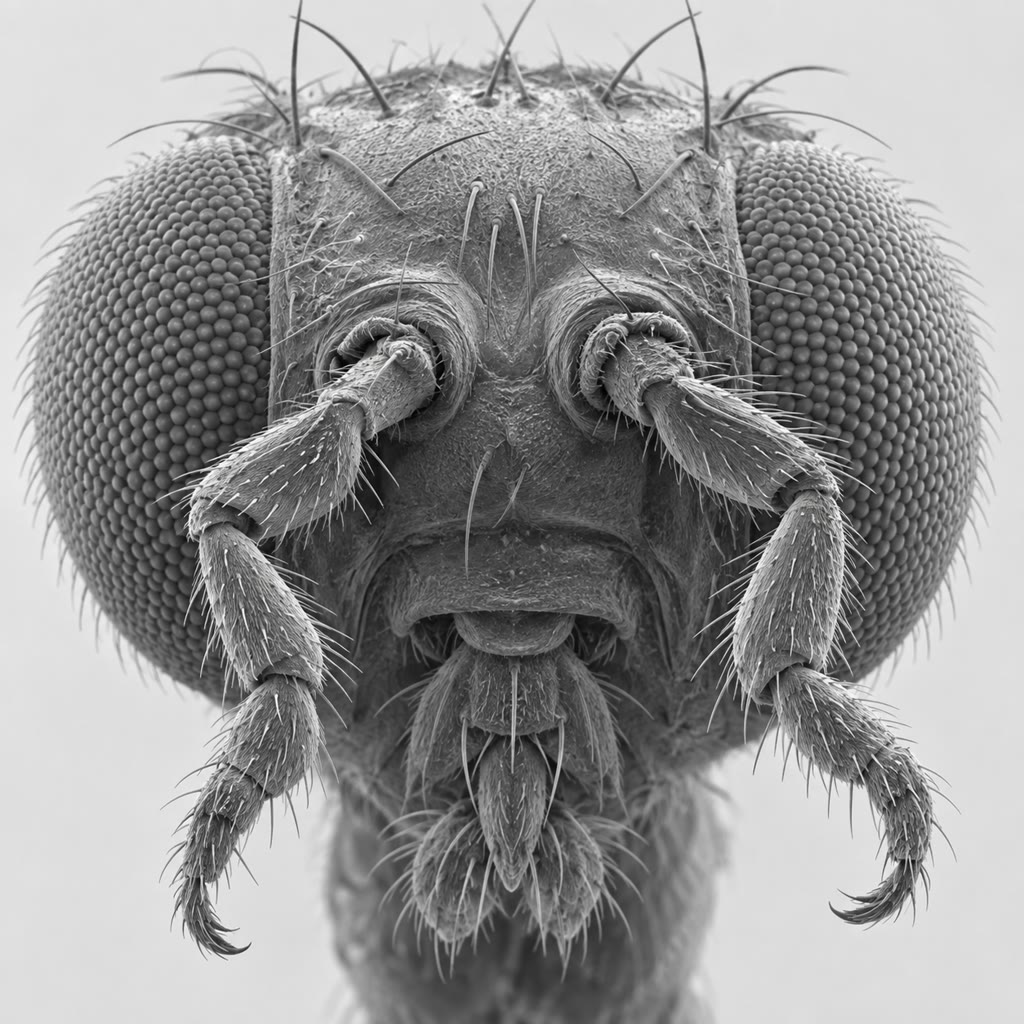
\includegraphics[width=0.34\linewidth]{images/book5/ai/b5-23-antennapedia-fly.jpg}\hspace{0.04\linewidth}
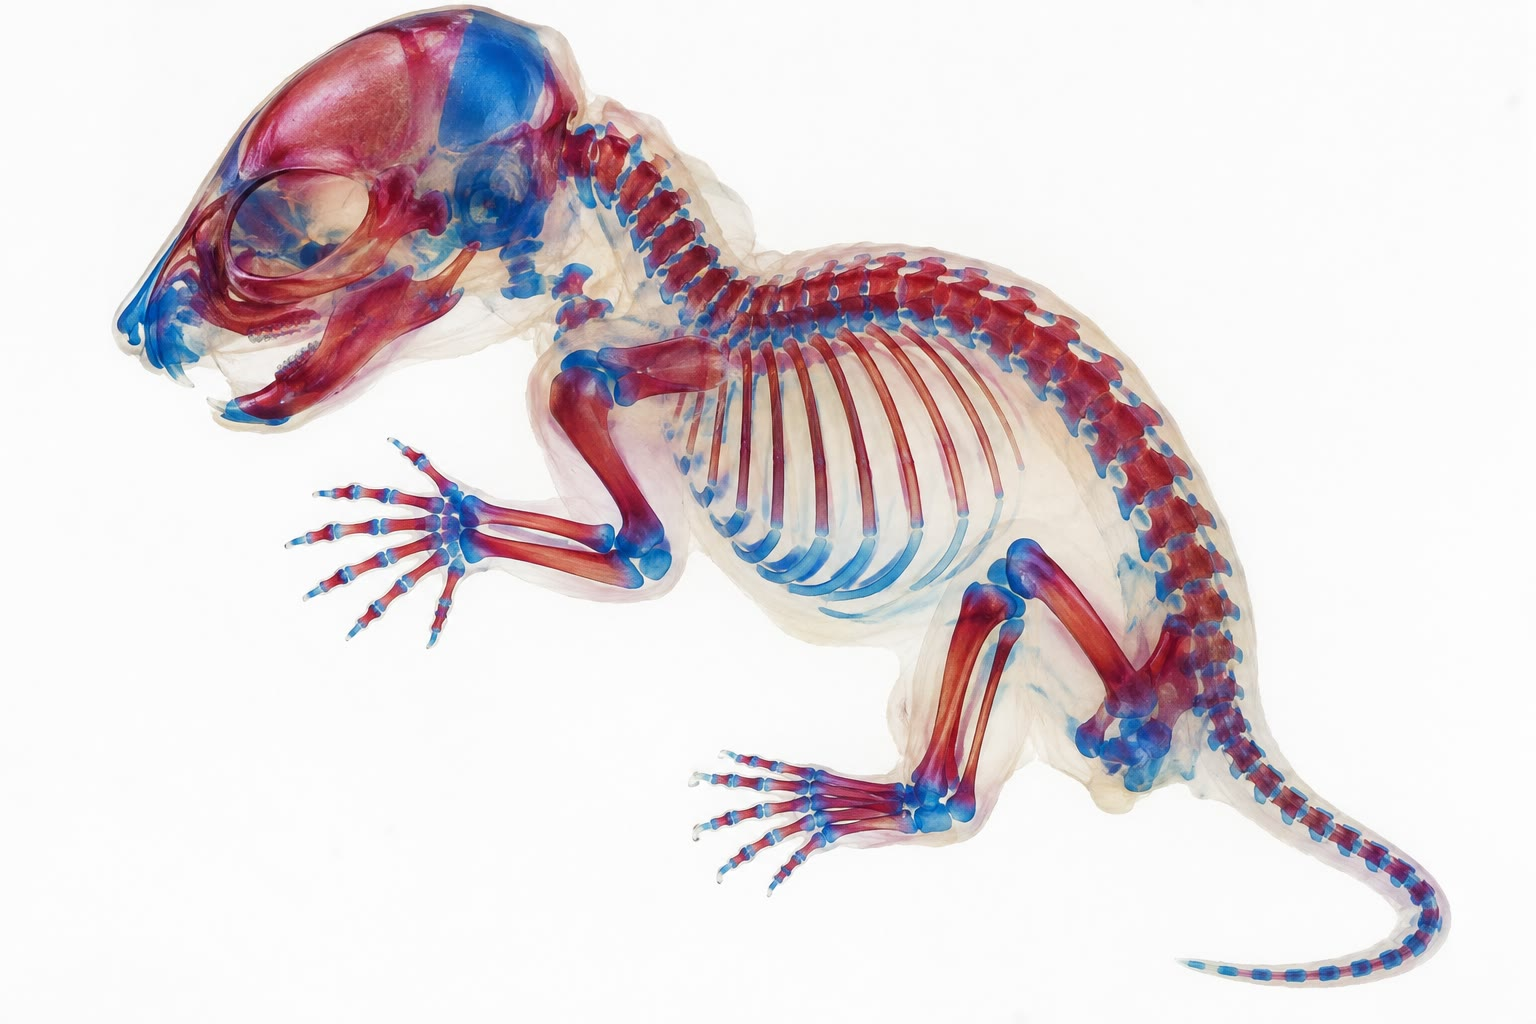
\includegraphics[width=0.5\linewidth]{images/book5/ai/b5-23-limb-skeleton-stain.jpg}

{\small बाएँ: किसी \emph{Antennapedia} उत्परिवर्ती मक्खी का सिर, जिसमें
स्पर्शश्रृंगों की जगह टाँगों की एक जोड़ी है --- यानी वह खंड ठीक बना और
उसे ग़लत पहचान बता दी गई। दाएँ: किसी चूहा-भ्रूण का कंकाल, जिसमें
उपास्थि नीली और अस्थि लाल है, और जिन कशेरुकाओं के अनुदिश वह \omterm{def:b3:developmental-genetics:hox}{Hox कूट}
पढ़ा जाता है।}
\end{omfigure}

\section{कोई कशेरुकी बनाना}

\begin{definition}[संगठक और संकेतन-केंद्र]\label{def:b3:developmental-genetics:organiser}
\index{संगठक}\index{प्रेरण}\index{सोनिक हेजहॉग}\index{उपांग-कलिका}\index{ध्रुवणकारी क्रियाशीलता का क्षेत्र}\index{शीर्षस्थ बाह्यचर्मी कटक}
कशेरुकी भ्रूण शुरू से ही कोशिकीय होते हैं, इसलिए उनकी प्रवणताएँ किसी
संकोशिका के विसरण के बजाय स्रवित प्रोटीनों से बनती हैं, और वही कुछ कुल
सब कुछ करते हैं: Wnt, Hedgehog, BMP तथा TGF-$\beta$ के दूसरे नातेदार,
FGF, Notch और रेटिनोइक अम्ल। श्पेमान और मांगोल्ड (1924) ने किसी न्यूट
गैस्ट्रुला के पृष्ठीय ओष्ठ का एक टुकड़ा किसी दूसरे के पेट पर कलमित किया
और सिर से पूँछ तक कोई दूसरा भ्रूण पाया, जो अधिकांशतः परपोषी कोशिकाओं का
बना था: वह कलम कोई \emph{संगठक} थी, जो अपने पड़ोसियों को कोई
तंत्रिका-तंत्र तथा अक्ष बनाने के लिए प्रेरित कर रही थी, और उसके अणु
सत्तर वर्ष बाद ऐसे स्रवित विरोधियों (कॉर्डिन, नॉगिन) के रूप में मिले जो
BMP रोकते हैं, और जिसकी अनुपस्थिति बाह्यचर्म को तंत्रिकीय बनने देती है
--- यानी वही चूक-अवस्था। फिर उस \emph{तंत्रिका नलिका} का पृष्ठ-अधर
प्रतिरूपण पृष्ठरज्जु तथा तल पट्टिका से आते \emph{सोनिक हेजहॉग} (ऊँचा:
प्रेरक न्यूरॉन; नीचा: \omterm{def:b3:nervous-systems:cells}{अंतर्न्यूरॉन}) और छत से आते BMP के बीच होता है; और
\emph{उपांग-कलिका} का दो केंद्रों से, यानी उसके पश्च किनारे पर बैठे उस
\emph{ध्रुवणकारी क्रियाशीलता के क्षेत्र} से जो Shh स्रवित करता है
(उसकी अग्र किनारे पर कलम अंगुलियों का कोई दर्पण-प्रतिबिंबी दुहराव देती
है, यानी अँगूठे से अँगूठा मिलाती छह अंगुलियाँ) और उसके सिरे पर बैठे उस
\emph{शीर्षस्थ बाह्यचर्मी कटक} से जो ऐसे FGF स्रवित करता है जो नीचे की
कोशिकाओं को बँटता रखते हैं और प्रगंडिका, प्रबाहु, हाथ का समीप-से-दूर का
क्रम निर्दिष्ट करते हैं। कलमन, उच्छेदन और प्रोटीन में भिगोए मनके अब भी
वही औज़ार हैं; और वह तर्क --- कोई स्थानीय स्रोत, कोई प्रवणता, देहलियाँ,
अनुलेखन कारकों का कोई कूट --- मक्खी वाला ही है।
\end{definition}

\begin{omfigure}
\begin{tikzpicture}[every node/.style={font=\scriptsize}, >=stealth]
  % limb bud
  \fill[omDef!12] (0,0) -- (0,3) .. controls (2.6,3.4) and (3.4,2.2) .. (3.4,1.5) .. controls (3.4,0.8) and (2.6,-0.4) .. (0,0) -- cycle;
  \draw[thick, omDef] (0,0) -- (0,3) .. controls (2.6,3.4) and (3.4,2.2) .. (3.4,1.5) .. controls (3.4,0.8) and (2.6,-0.4) .. (0,0);
  \draw[very thick, omMeth!70!black] (2.9,2.5) .. controls (3.45,1.9) and (3.45,1.1) .. (2.9,0.5);
  \node[right, align=left, omMeth!70!black, font=\tiny] at (3.5,1.5) {शीर्षस्थ बाह्यचर्मी कटक:\\FGF8; प्रगति-क्षेत्र को\\बँटता रखता है;\\समीप $\to$ दूर};
  \begin{scope}
    \clip (0,0) -- (0,3) .. controls (2.6,3.4) and (3.4,2.2) .. (3.4,1.5) .. controls (3.4,0.8) and (2.6,-0.4) .. (0,0) -- cycle;
    \foreach \i/\op in {1/50, 2/38, 3/26, 4/14} { \draw[omThm!\op, thick] (0.6,0.5) circle ({0.45*\i}); }
  \end{scope}
  \fill[omThm!50] (0.6,0.5) ellipse (0.5 and 0.35); \node[anchor=north, align=center, omThm, font=\tiny] at (0.9,-0.2) {ZPA: सोनिक हेजहॉग,\\पश्च $\to$ अग्र};
  \node[left, font=\tiny] at (-0.05,2.6) {अग्र}; \node[left, font=\tiny] at (-0.05,0.4) {पश्च};
  \node[left, font=\tiny] at (-0.05,1.5) {देह-भित्ति};
  \draw[->, thick] (0.3,1.5) -- (3.0,1.5); \node[above, font=\tiny] at (1.75,1.55) {प्रगंडिका, प्रबाहु, अंगुलियाँ};
  % right: digit code
  \node[right, align=left] at (7.2,2.6) {Shh के संसर्ग से अंगुली की पहचान:\\अँगूठा (अंगुली 1): कोई नहीं;\\अंगुली 2--3: प्रवणता;\\अंगुली 4--5: Shh बनाती कोशिकाओं से};
  \node[right, align=left] at (7.2,1.0) {अग्र में कोई दूसरा ZPA कलमित कीजिए:\\दर्पण-प्रतिबिंबी दुहराव, 4-3-2-2-3-4;\\Shh प्रोटीन का मनका भी वही करता है};
  \node[right, align=left, gray] at (7.2,-0.2) {वही अणु तंत्रिका नलिका का\\(जहाँ ऊँचा है वहाँ प्रेरक न्यूरॉन) और आँत का प्रतिरूपण करता है};
\end{tikzpicture}

{\small \omterm{def:b3:developmental-genetics:organiser}{उपांग-कलिका} के दो संकेतन-केंद्र। पश्च किनारे से आता \omterm{def:b3:developmental-genetics:organiser}{सोनिक
हेजहॉग} कोशिकाओं को बताता है कि कौन-सी अंगुली बनना है; और सिरे से आता
FGF उन्हें बताता है कि वे उस उपांग पर कितनी दूर हैं। जो कलमें किसी
केंद्र को हिला देती हैं वे उस प्रतिरूप को भी साथ हिला देती हैं।}
\end{omfigure}

\begin{proposition}[स्वतःस्फूर्त प्रतिरूप: ट्यूरिंग का तंत्र]\label{prop:b3:developmental-genetics:turing}
\index{ट्यूरिंग प्रतिरूप}\index{अभिक्रिया--विसरण}\index{सक्रियक--निरोधक}
हर प्रतिरूप किसी पहले से मौजूद प्रवणता से नहीं पढ़ा जाता। ट्यूरिंग
(1952) ने दिखाया कि दो ऐसे विसरित होते पदार्थ जो अभिक्रिया करें ---
कोई \emph{सक्रियक}, जो अपना ही और किसी \emph{निरोधक} का उत्पादन बढ़ाए,
और कोई निरोधक, जो उस सक्रियक को दबाए और कहीं तेज़ विसरित हो --- किसी
एकसमान क्षेत्र को स्वतःस्फूर्त ढंग से शिखरों की किसी नियमित सरणी में
बदल सकते हैं: सक्रियक की कोई छोटी स्थानीय अधिकता स्वयं-वर्धन से बढ़ती
है जबकि जो निरोधक वह बनाती है वह फैल जाता है और पास कोई नया शिखर बनने
से रोक देता है, इसलिए शिखर किसी ऐसे अंतराल पर प्रकट होते हैं जो उस
निरोधक की पहुँच तय करती है,
$\lambda \sim \sqrt{D_{\text{निरोधी}}/k_{\text{निरोधी}}}$, न कि कोई बाहरी
निर्देशांक। वह तंत्र, जिसका गणित यहाँ स्वीकार कर लिया गया है, प्राणियों
की खालों के धब्बों तथा धारियों, रोम-पुटकों और पंख-कलिकाओं के अंतराल,
तालु की कटकों, हाथ की अंगुलियों (जिनकी संख्या तब बढ़ जाती है जब Hox की
क्रियाशीलता घटाकर उस प्रतिरूप का तरंगदैर्घ्य छोटा कर दिया जाए), और
ज़ेब्राफ़िश की धारियों का सबसे अच्छा हिसाब है, जहाँ वे अंतःक्रिया करती
कोशिकाएँ --- यानी ऐसी वर्णक कोशिकाएँ जो एक तरह के पड़ोसियों को दूर
धकेलती हैं और दूसरी तरह के को दूर से खींचती हैं --- पहचान ली गई हैं और
उनकी धारियाँ लेज़र-उच्छेदन के बाद ठीक वैसे फिर बना दी गई हैं जैसा वह
सिद्धांत पूर्वानुमान करता है।
\end{proposition}
\admitted

\section{आकार का विकास}

\begin{definition}[विकास-परिवर्धन]\label{def:b3:developmental-genetics:evodevo}
\index{गहन समजातता}\index{आनुवंशिक औज़ार-पेटी}\index{सिस-नियामक विकास}\index{विषमकालिकता}
जो जीन प्राणी बनाते हैं वे कोई प्राचीन और साझा \emph{औज़ार-पेटी} हैं:
कुछ सौ अनुलेखन कारक और संकेतन-पथ, जो सारे प्राणियों के साझा पूर्वज में
मौजूद थे, और प्राणी-विविधता अधिकांशतः इस बदलाव से आती है कि वे
\emph{कब, कहाँ और कितने} अभिव्यक्त होते हैं, न कि इससे कि वे क्या
कूटबद्ध करते हैं। \emph{गहन समजातता}: जीन \emph{Pax6} मक्खियों,
स्क्विडों और चूहों में नेत्र-निर्माण संचालित करता है, जिनकी आँखें अंगों
के रूप में समजात नहीं हैं --- और किसी मक्खी की टाँग पर अभिव्यक्त चूहे का
\emph{Pax6} वहाँ कोई अस्थानिक मक्खी-आँख बना देता है (हाल्डर, गेरिंग,
1995)। \emph{सिस-नियामक विकास}: मीठे पानी के स्टिकलबैकों में श्रोणी-शूलों
का लोप \emph{Pitx1} जीन के किसी एक संवर्धक का विलोपन है, जबकि वह
प्रोटीन अछूता है और कहीं और अब भी काम कर रहा है; कुछ फल-मक्खियों में
पंख-धब्बों का लोप \emph{yellow} के किसी संवर्धक का बदलाव; और साँपों में
टाँगों का लोप उपांग में \emph{sonic hedgehog} का कोई टूटा संवर्धक।
\emph{Hox खिसकाव}: \emph{Hoxc6} की अभिव्यक्ति-सीमा चूहे, चूज़े, हंस और
साँप, सबमें पहली वक्षीय कशेरुका चिह्नित करती है, क्रमशः कशेरुका 7, 14,
23 और 3 पर; और कीटों में उदरीय टाँगों का लोप Hox प्रोटीन Ubx का कोई ऐसा
दमनकारी प्रांत पा लेना था जो टाँग-जीन \emph{Distal-less} बंद कर देता
है, जबकि क्रस्टेशियनों में वह नहीं करता। \emph{विषमकालिकता}, यानी किसी
परिवर्धनी कार्यक्रम के समय का कोई बदलाव, ने ऐक्सोलोटल को कोई स्थायी
डिंभ बना दिया और मानव चेहरे को किसी किशोर कपि का। यह पुराना प्रश्न कि
नए आकार कैसे उठते हैं अब नियामक DNA का प्रश्न बन जाता है: जीनोम का
अधिकांश, जो आकार के लिए मायने रखता है, जीन नहीं बल्कि स्विच है।
\end{definition}

\begin{example}[चार पंख]\label{ex:b3:developmental-genetics:four-wings}
मक्खियों के पूर्वजों के चार पंख थे, जैसे व्याध-पतंगों और मधुमक्खियों के
अब भी हैं; मक्खियों के दो हैं, और पिछली जोड़ी घटकर संतुलक रह गई।
मक्खियों में \emph{Ultrabithorax} तीसरे वक्षीय खंड में अभिव्यक्त होता है
और वहाँ पंख-कार्यक्रम दबा देता है --- यानी कोई सौ लक्ष्य जीन, और कोई
हॉल्टियर उन्हीं जीनों के बंद कर दिए जाने वाला कोई पंख। लुइस की तिहरी
उत्परिवर्ती मक्खी, जिसके तीसरे खंड में \emph{Ubx} का प्रकार्य न हो,
पंखों की कोई दूसरी जोड़ी उगा लेती है: यानी कोई नई संरचना नहीं, बल्कि
किसी पुरानी की रिहाई। तितलियों में \emph{Ubx} पश्च-पंख में भी अभिव्यक्त
होता है, और वहाँ वह उस पंख को दबाता नहीं बल्कि उसका प्रतिरूप बदल देता
है: यानी वही प्रोटीन, लक्ष्यों का कोई भिन्न समुच्चय। द्विपंखी विकास के
चालीस करोड़ वर्ष किसी एक खंड में किसी एक जीन के निर्णय पर टिके रहे, और
कोई एक उत्परिवर्तन उसे किसी एक पीढ़ी में उलट देता है --- और इसीलिए आकार
का इतिहास उन्हीं जीनों में पढ़ा जा सकता है जो उसे बनाते हैं।
\end{example}

\begin{remark}[रसायन से ज्यामिति]\label{rem:b3:developmental-genetics:remark}
किसी भ्रूण के पास न कोई नक़्शा है न कोई सर्वेक्षक। उसके पास विसरण तथा
क्षय से बनी कुछ प्रवणताएँ हैं, ऐसी कोशिकाएँ हैं जो उन्हें देहलियों के
सामने पढ़कर अनुलेखन कारक चालू कर देती हैं, और उन कारकों का कोई ऐसा कूट
जो हर क्षेत्र को बताता है कि उसे क्या बनना है; उसके पास ऐसे स्थानीय
\omterm{def:b3:developmental-genetics:organiser}{संगठक} हैं जो अपने पड़ोसियों को प्रेरित करते हैं, और ऐसी अभिक्रियाएँ जो
स्वयं का प्रतिरूपण कर लेती हैं। वह गणित प्रथम-कोटि बलगतिकी और विसरण का
है --- कोई चरघातांक, कोई वर्गमूल, कोई देहली --- और वह न केवल यह समझाता
है कि किसी मक्खी का सिर कहाँ रखा जाता है, बल्कि यह भी कि किसी जीन को
दुगुना करने से कोई सीमा किसी नियत दूरी से क्यों खिसकती है, कोई संकेत
दुहराने पर छह अंगुलियाँ क्यों प्रकट होती हैं, और किसी साँप की तीन सौ
पसलियाँ क्यों होती हैं। विकास उन स्विचों का संपादन करता है, उस यंत्र का
नहीं: किसी स्पंज और किसी मनुष्य की औज़ार-पेटी लगभग वही है, और जो भिन्न
है वह तारबंदी है।
\end{remark}

\section{अभ्यास}

\begin{exercise}[$\star$]\label{exo:b3:developmental-genetics:1}
मक्खी की खंडन-पदानुक्रमी की चारों तहें बताइए, हर एक का एक-एक जीन, और वह
उत्परिवर्ती लक्षणरूप जिसने उसे उसके वर्ग में रखा।
\end{exercise}

\begin{exercise}[$\star$]\label{exo:b3:developmental-genetics:2}
\omterm{def:b3:developmental-genetics:hierarchy}{मातृ-प्रभाव जीन} क्या है? किसी \emph{bicoid} विहीनकारी उत्परिवर्तन के
लिए समयुग्मजी किसी मादा का संगम किसी वन्य-प्ररूपी नर से कराया जाता है:
उसके भ्रूणों का वर्णन कीजिए और समझाइए कि उनका अपना जीनरूप उन्हें क्यों
नहीं बचाता।
\end{exercise}

\begin{exercise}[$\star$]\label{exo:b3:developmental-genetics:3}
\omterm{def:b3:developmental-genetics:hox}{सहरैखिकता} और पश्च प्रबलता बताइए। \emph{Hoxc8}-विहीन किसी चूहे के और
अपने सिर में \emph{Antennapedia} अभिव्यक्त करती किसी मक्खी के लक्षणरूप
का पूर्वानुमान कीजिए।
\end{exercise}

\begin{exercise}[$\star$]\label{exo:b3:developmental-genetics:4}
श्पेमान--मांगोल्ड कलम ने क्या दिखाया, और उस \omterm{def:b3:developmental-genetics:organiser}{संगठक} के अणु क्या निकले?
तंत्रिकीय भवितव्य को ``चूक-अवस्था'' क्यों कहते हैं?
\end{exercise}

\begin{exercise}[$\star\star$]\label{exo:b3:developmental-genetics:5}
Bicoid: $D = \qty{4}{\micro m^2/s}$, अर्ध-आयु काल \qty{35}{min}।
$k$, $\lambda$, और अग्र ध्रुव पर तथा अंडे के बीच
(\qty{250}{\micro m}) की सांद्रताओं का अनुपात निकालिए।
\end{exercise}

\begin{exercise}[$\star\star$]\label{exo:b3:developmental-genetics:6}
$\lambda = \qty{100}{\micro m}$ के साथ, कोई सीमा
\qty{240}{\micro m} पर बैठी है। यदि उस माँ के पास \emph{bicoid} की दो
के बजाय चार प्रतियाँ हों तो वह कहाँ बैठती है? एक प्रति? उन खिसकावों को
\qty{500}{\micro m} के अंडे के अंश के रूप में लिखिए।
\end{exercise}

\begin{exercise}[$\star\star$]\label{exo:b3:developmental-genetics:7}
कोरकचर्म पर केंद्रक \qty{8}{\micro m} की दूरी पर हैं।
$\lambda = \qty{100}{\micro m}$ के साथ किसी सीमा को किसी एक केंद्रक के
भीतर रखने के लिए, किसी केंद्रक को Bicoid की सांद्रता कितनी परिशुद्धि से
पढ़नी पड़ेगी? यदि वह केंद्रक किसी काल $\tau$ भर अणु गिने और वह गिनती
प्वासों हो, तो उसे कितने गिनने पड़ेंगे?
\end{exercise}

\begin{exercise}[$\star\star$]\label{exo:b3:developmental-genetics:8}
वह प्रवणता स्थायी अवस्था तक काल-मापक्रम $1/k$ पर पहुँचती है।
\qty{35}{min} के अर्ध-आयु काल के साथ, \qty{60}{min}, \qty{90}{min} और
\qty{120}{min} पर स्थायी-अवस्था सांद्रता का कितना अंश छू लिया जाता है?
किसी ऐसे भ्रूण के लिए, जिसे वह प्रवणता \qty{150}{min} तक पढ़नी हो, इससे
क्या निकलता है?
\end{exercise}

\begin{exercise}[$\star\star$]\label{exo:b3:developmental-genetics:9}
किसी चूज़े की \omterm{def:b3:developmental-genetics:organiser}{उपांग-कलिका} के अग्र किनारे पर कोई ZPA कलमित की जाती है।
अंगुली-प्रतिरूप का पूर्वानुमान कीजिए, और वह प्रतिरूप भी जो तब मिलता यदि
उसके बजाय वहाँ Shh की कोई कम मात्रा छोड़ता कोई मनका बैठाया जाता।
\end{exercise}

\begin{exercise}[$\star\star\star$]\label{exo:b3:developmental-genetics:10}
कोई आकारजन लंबाई $L$ के किसी ऊतक भर में प्रति एकांक आयतन दर $s$ से बनता
है, दर $k$ से अपघटित होता है, और सीमा $x =
L$ पर नष्ट कर दिया जाता है (कोई अवशोषी गर्त), और $x = 0$ पर कोई फ्लक्स
नहीं। $Dc'' - kc + s =
0$ को $c(x)$ के लिए हल कीजिए और उसका रेखाचित्र बनाइए। इस प्रवणता का आकार किसी-एक-सिरे-पर-स्रोत
वाली स्थिति से कैसे भिन्न है, और $L \ll \lambda$ होने पर क्या होता है?
\end{exercise}

\begin{exercise}[$\star\star\star$]\label{exo:b3:developmental-genetics:11}
$T_{1} = 0.3c_{0}$ और $T_{2} = 0.08c_{0}$ पर दो देहलियाँ किसी प्रवणता
को तीन क्षेत्रों में बाँट देती हैं। दिखाइए कि पहले दो क्षेत्रों की
चौड़ाइयाँ $c_{0}$ पर निर्भर नहीं हैं, और समझाइए कि जिस भ्रूण की
\emph{लंबाई} व्यष्टियों के बीच बदलती हो (\qty{450}{} से
\qty{550}{\micro m}) उसे अपना प्रतिरूप मापक्रमित करने के लिए किसी एक
चरघातांक से अधिक कुछ क्यों चाहिए। कोई एक तंत्र सुझाइए।
\end{exercise}

\begin{exercise}[$\star\star\star$]\label{exo:b3:developmental-genetics:12}
स्टिकलबैकों ने \emph{Pitx1} का कोई संवर्धक विलोपित करके श्रोणी-शूल खोए,
और साँपों ने \emph{sonic hedgehog} का कोई संवर्धक तोड़कर उपांग। समझाइए
कि किसी खोई या बदली संरचना तक का आम रास्ता कूटलेखी बदलावों के बजाय
नियामक बदलाव क्यों हैं, और यह बहुप्रभाविता के हिसाब से तथा इस हिसाब से
कि वही प्रोटीन कहीं और क्या करता है।
\end{exercise}

\section{समस्या: फ़्रांसीसी झंडा}

\begin{problem}[{सप्तांत समस्या --- प्रथम-कोटि बलगतिकी से गणित किया गया
किसी अंडे का निर्देशांक-तंत्र: Bicoid प्रवणता की लंबाई, स्रोत और बनने
का समय, वे सीमाएँ जो वह खींचती है और उनकी परिशुद्धि, जीन-मात्रा तथा
अंडे का आकार उनका क्या करते हैं, और अनुवर्ती पढ़ा गया Hox कूट, जिसका
अंत क्षय-लंबाई पर होता है, प्रति दुगुनी खिसकाव पर, और स्थानिक परिशुद्धि
पर}]
\label{pb:b3:developmental-genetics:1}
आँकड़े: अंडे की लंबाई \qty{500}{\micro m}; Bicoid $D = \qty{4}{\micro m^2/s}$,
अर्ध-आयु काल \qty{35}{min}; स्रोत-फ्लक्स ऐसा कि दो मातृ प्रतियों के साथ
$c_{0} = \qty{50}{nM}$; चक्र 14 पर केंद्रकों का अंतराल
\qty{8.5}{\micro m}; दो-प्रति स्थिति के लिए देहलियाँ
$T_{1} = 0.3\,c_{0}$ (सिर/वक्ष) और $T_{2} =
0.08\,c_{0}$ (\emph{hunchback} सीमा)। किसी एक केंद्रक के लिए पठन-शोर
$\delta c/c = 0.1$। आवोगाद्रो संख्या
\qty{6e23}{}; कोई केंद्रक \qty{3}{\micro m} त्रिज्या का गोला है।

\medskip
\noindent\textbf{भाग I --- वह प्रवणता।}
\begin{enumerate}
  \item अर्ध-आयु काल से $k$ निकालिए, \unit{s^{-1}} में, और जीवनकाल
        $1/k$ मिनटों में।
  \item $\lambda = \sqrt{D/k}$ माइक्रोमीटरों में निकालिए। वह अंडा कितनी
        क्षय-लंबाइयों का है?
  \item सांद्रता ध्रुव से ध्रुव तक कितने गुना गिरती है? अंडे के बीच
        किसी एक केंद्रक-अंतराल भर कितने गुना?
  \item स्रोत-फ्लक्स $J = c_{0}\sqrt{Dk}$
        \unit{nM\,\micro m\,s^{-1}} में निकालिए, और अग्र ध्रुव के
        \qty{1}{\micro m^2} टुकड़े में प्रति सेकंड घुसते अणुओं की
        संख्या।
  \item ध्रुव पर ($c_{0}$) और अंडे के बीच किसी केंद्रक में Bicoid
        अणुओं की संख्या।
  \item \qty{60}{min} और \qty{120}{min} पर छू ली गई स्थायी अवस्था का
        अंश ($1 - \mathrm{e}^{-kt}$)। लगभग \qty{120}{min} पर, जब वे
        सीमाएँ खींची जाती हैं, क्या वह प्रवणता स्थायी है?
\end{enumerate}

\medskip
\noindent\textbf{भाग II --- सीमाएँ।}
\begin{enumerate}[resume]
  \item दोनों सीमाओं की स्थितियाँ, \unit{\micro m} में और अंडे की
        लंबाई के अंशों के रूप में।
  \item उस माँ के पास चार प्रतियाँ हैं: नया $c_{0}$, और दोनों सीमाओं की
        स्थितियाँ। हर एक कितना खिसकी? छह प्रतियाँ?
  \item एक प्रति: स्थितियाँ। कौन-से क्षेत्र बढ़े, कौन-से सिकुड़े?
  \item \qty{10}{\%} के पठन-शोर से स्थानिक त्रुटि, माइक्रोमीटरों में
        और केंद्रक-अंतरालों में।
  \item यदि वह त्रुटि एक केंद्रक भर होनी चाहिए, तो कौन-सी पठन-परिशुद्धि
        चाहिए? यदि वह केंद्रक $n$ स्वतंत्र पठनों का औसत ले और वह शोर
        $1/\sqrt{n}$ की तरह गिरे, तो कितने पठन?
  \item \emph{hunchback} की सीमा पर बैठा कोई केंद्रक प्रश्न~5 में
        निकाली गई संख्या रखता है। किसी एक तात्क्षणिक गिनती का प्वासों
        शोर $1/\sqrt{N}$ क्या है? \qty{10}{\%} से तुलना कीजिए और
        टिप्पणी कीजिए।
\end{enumerate}

\medskip
\noindent\textbf{भाग III --- मापक्रमण और मज़बूती।}
\begin{enumerate}[resume]
  \item अंडे \qty{450}{} से \qty{550}{\micro m} तक बदलते हैं। यदि
        $\lambda$ तथा $c_{0}$ नियत हों, तो हर एक में
        \emph{hunchback} की सीमा अंडे की लंबाई के किस अंश पर पड़ती है?
        क्या वह प्रतिरूप मापक्रमित है?
  \item इसके बजाय मान लीजिए कि $D$ $L^{2}$ की तरह मापक्रमित होता है
        (वही जीवनकाल, पर कोई ऐसा स्रोत जिसका फैलाव उस अंडे के साथ
        बढ़ता है)। दिखाइए कि तब $\lambda/L$ अचर है और वह प्रतिरूप
        मापक्रमित होता है। क्या यह प्रशंसनीय है?
  \item \emph{hunchback} जीन Bicoid पर $5$ के \omterm{def:b3:structural-biology:allostery}{हिल गुणांक} से अनुक्रिया
        देता है: उसकी अभिव्यक्ति $c^{5}/(c^{5} + T^{5})$ है। उस सीमा
        के आसपास अभिव्यक्ति \qty{10}{\%} से \qty{90}{\%} तक कितने
        माइक्रोमीटरों में जाती है? किसी एक केंद्रक-अंतराल से तुलना
        कीजिए।
  \item समझाइए कि कोई तीखी अनुक्रिया किसी सीमा को तीखा तो करती है पर
        सांद्रता-शोर से आती स्थानिक त्रुटि को अपने आप क्यों नहीं घटाती।
  \item रिक्ति-जीनों के बीच का पारस्परिक दमन उनकी सीमाएँ तीखी तथा
        स्थिर करता है। एक वाक्य में तर्क दीजिए कि जो दो जीन एक-दूसरे का
        दमन करें वे किसी एक ही केंद्रक में स्थायी अवस्था पर दोनों चालू
        क्यों नहीं रह सकते।
  \item तापमान $D$ को प्रति अंश \qty{2}{\%} और $k$ को \qty{6}{\%}
        बढ़ा देता है। प्रति अंश $\lambda$ में बदलाव, और
        \qty{5}{\celsius} गरम किसी कमरे के लिए सीमा का खिसकाव। भ्रूणों
        को कोई भरपाई करता तंत्र क्यों चाहिए हो सकता है?
\end{enumerate}

\medskip
\noindent\textbf{भाग IV --- पहचान।}
\begin{enumerate}[resume]
  \item \omterm{def:b3:developmental-genetics:hox}{Hox कूट}: मक्खी के आठ \omterm{def:b3:developmental-genetics:hox}{Hox जीनों} में से हर एक के चालू या बंद
        होने पर कितने कूट संभव हैं? कितने काम में आते हैं (चौदह खंड)?
        पश्च प्रबलता उस प्रभावी संख्या को क्यों घटा देती है?
  \item किसी मक्खी के तीसरे वक्षीय खंड में \emph{Ubx} नहीं है। वह खंड
        क्या बन जाता है, और उसका परिणाम कोई नई संरचना नहीं बल्कि चार
        पंख क्यों है?
  \item किसी चूहे की \emph{Hoxc6} सीमा कशेरुका 7 पर पड़ती है और किसी
        हंस की 23 पर। इससे उनकी गर्दनों के बारे में क्या पूर्वानुमान
        निकलता है, और विकास में क्या बदला: वह जीन, या उसकी
        अभिव्यक्ति?
  \item कोई ZPA कलम अंगुलियाँ 4-3-2-2-3-4 देती है। बीच में मिलती दो
        Shh प्रवणताओं से उस प्रतिरूप की व्याख्या कीजिए।
  \item हाल्डर और गेरिंग ने किसी मक्खी की टाँग में चूहे का \emph{Pax6}
        अभिव्यक्त किया और वहाँ कोई मक्खी-आँख पाई। इससे उस जीन के बारे
        में क्या पता चलता है, और मक्खियों तथा चूहों की आँखों के बारे
        में क्या \emph{नहीं} पता चलता?
  \item छठी अंगुली: ट्यूरिंग का तरंगदैर्घ्य छोटा करने से एक अंगुली जुड़
        जाती है। \qty{2}{mm} की किसी हाथ-पट्टिका भर पाँच अंगुलियों के
        साथ, कौन-सा तरंगदैर्घ्य-बदलाव छह देता है? उस अभिक्रिया--विसरण
        तंत्र का कौन-सा प्राचल उसे पैदा करता?
  \item सारांश दीजिए: $\lambda$ (प्रश्न~2), स्रोत के दुगुने होने पर
        सीमा का खिसकाव (प्रश्न~8), और \qty{10}{\%} शोर से आती स्थानिक
        त्रुटि (प्रश्न~10)।
\end{enumerate}
\end{problem}
